
%\chapter{Methode} % Main chapter title
%\label{chapter3:Methode} % Change X to a consecutive number; for referencing this chapter elsewhere, use \ref{ChapterX}


%-----------------------------------
% SUBSECTION "Sniffer"
%-----------------------------------

\section{Sniffer Device}
\textcolor{red}{Kapitel nochmals durchlesen!}\\
% \textcolor{red}{Was ist ein Sniffer}\\
% Ein Sniffer ist grundsätzlich ein Gerät oder ein Software-Tool welches die Kommunikation zweier oder mehrerer Geräten überwachen und aufzeichnen kann.

% Ein solcher Sniffer wird Beispielsweise oft eingesetzt um den Netzwerkverkehr zu überwachen. Ein bekanntes Beispiel eines Sniffers dieser Art ist die Sniffer-Software Wireshark.\\

% Der Sniffer wie er auch in dieser Projektarbeit entwickelt wird, ist Physisch und wird direkt an einen Datenbus gehängt um von diesem lesen zu können.
% Dabei fängt der Sniffer die versendeten Datenpakete auf dem Bus ab ohne jegliche Störungen oder
% Einschränkungen der Kommunikation der Geräte zu verursachen.

Ein Sniffer ist ein Gerät oder Software-Tool, das in der Lage ist, die Kommunikation zwischen zwei
oder mehreren Geräten zu überwachen und aufzuzeichnen. Diese Art von Werkzeug wird häufig verwendet,
um den Datenverkehr in Netzwerken oder auf Kommunikationsbussen zu analysieren.

Ein bekanntes Beispiel für ein solches Sniffer-Tool ist die Software Wireshark, die weit verbreitet
zur Überwachung von Netzwerkprotokollen eingesetzt wird.

Im Rahmen dieser Projektarbeit wird ein physischer Sniffer entwickelt, der direkt an einen Datenbus
angeschlossen wird, um die auf dem Bus übertragenen Datenpakete zu lesen. Dabei agiert der Sniffer
passiv und erfasst die übertragenen Daten, ohne die Kommunikation zwischen den Geräten zu beeinflussen
oder zu stören.

%--------------------------------------------------------------------------------
% SECTION Stand von Konkurenzprodukten
%--------------------------------------------------------------------------------

\section{Recherche bestehende Produkte}
\label{sec:recherche}

In einer Recherche zu bereits auf dem Markt vorhandenen MVB-Sniffern wurden verschiedene Varianten
gefunden. Teilweise wurden Anforderungen, die an den zu entwickelten Sniffer gestellt wurden, erfüllt.
Es wurden drei Geräte gewählt welche in diesem Kapitel etwas näher vorgestellt werden. In Tabelle
\ref{tab:mvb_analyzer} sind dazu die verschiedenen Geräte mit dessen Merkmalen aufgelistet.
Abschliessend wird in diesem Unterkapitel darauf eingegangen was den Sniffer, welcher entwickelt
werden soll, ausmacht und welchen Vorteil dieser in der künftigen Anwendung bringen soll.

\begin{table}[h!]
    \centering
    \begin{tabular}{|>{\raggedright\arraybackslash}p{3cm}|>{\raggedright\arraybackslash}p{3cm}|>{\raggedright\arraybackslash}p{3cm}|>{\raggedright\arraybackslash}p{3cm}|>{\raggedright\arraybackslash}p{3cm}|}
        \hline
        \textbf{Name} & \textbf{AMiT MVB Analyzer} & \textbf{Ci4Rail MIO03 MVB/CAN Sniffer} & \textbf{Yacer MVB-Analyzer Protocol Analyzer} \\
        \hline
        \textbf{Interface Typen} & EMD / ESD & & \\
        \hline
        \textbf{Galvanische Trennung} & Ja & & \\
        \hline
        \textbf{Connectors} & 2 × D-Sub DE-9, RJ45,  & & \\
        \hline
        \textbf{Communication Rate MVB} & 1.5 Mbps ±0.01 \% & & \\
        \hline
        \textbf{Communication Rate Endgerät} & ETH: 10 / 100 Mbps & & \\
        \hline
        \textbf{Spannungs-versorgung} & 16,8 V - 33,6 V DC & & \\
        \hline
        \textbf{Gewicht} & 0,9 kg & & \\
        \hline
        \textbf{Dimensionen (b × h × l)} & (33 × 228 × 87) mm & & \\
        \hline
        \textbf{Analyse Tool} & WireShark & & \\
        \hline
    \end{tabular}
    \caption{Vergleich MVB Sniffer}
    \label{tab:mvb_analyzer}
\end{table}

%-----------------------------------
% SUBSECTION "Amit"
%-----------------------------------
\newpage
\subsection{Konkurenz 1 (Amit Transportation)}
\textcolor{red}{Amit MVB Analyzer}

\begin{figure}[H]
    \centering
    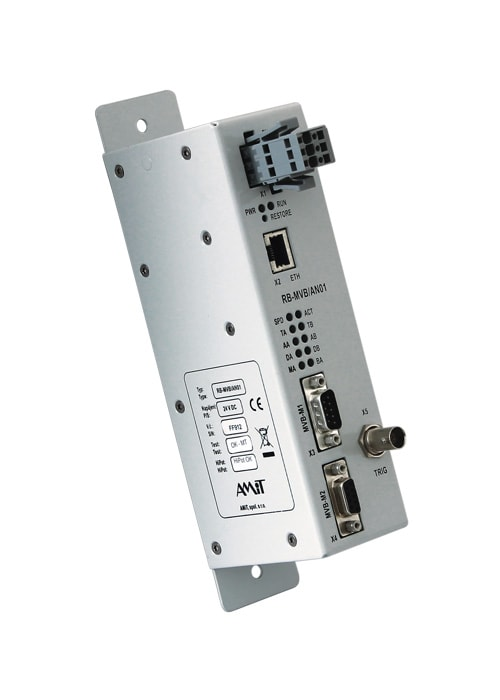
\includegraphics[width=0.4\linewidth]{Figures/Chap3/Konkurenz/Amit.jpg}
    \caption{Bild von Herstellerseite}
    \label{fig:AmitAnalyzer}
\end{figure}


%-----------------------------------
% SUBSECTION "Ci4Rail"
%-----------------------------------

\subsection{Konkurenz 2 (Ci4Rail)}
\textcolor{red}{IP\ Based\ Sniffer}

\begin{figure}[H]
    \centering
    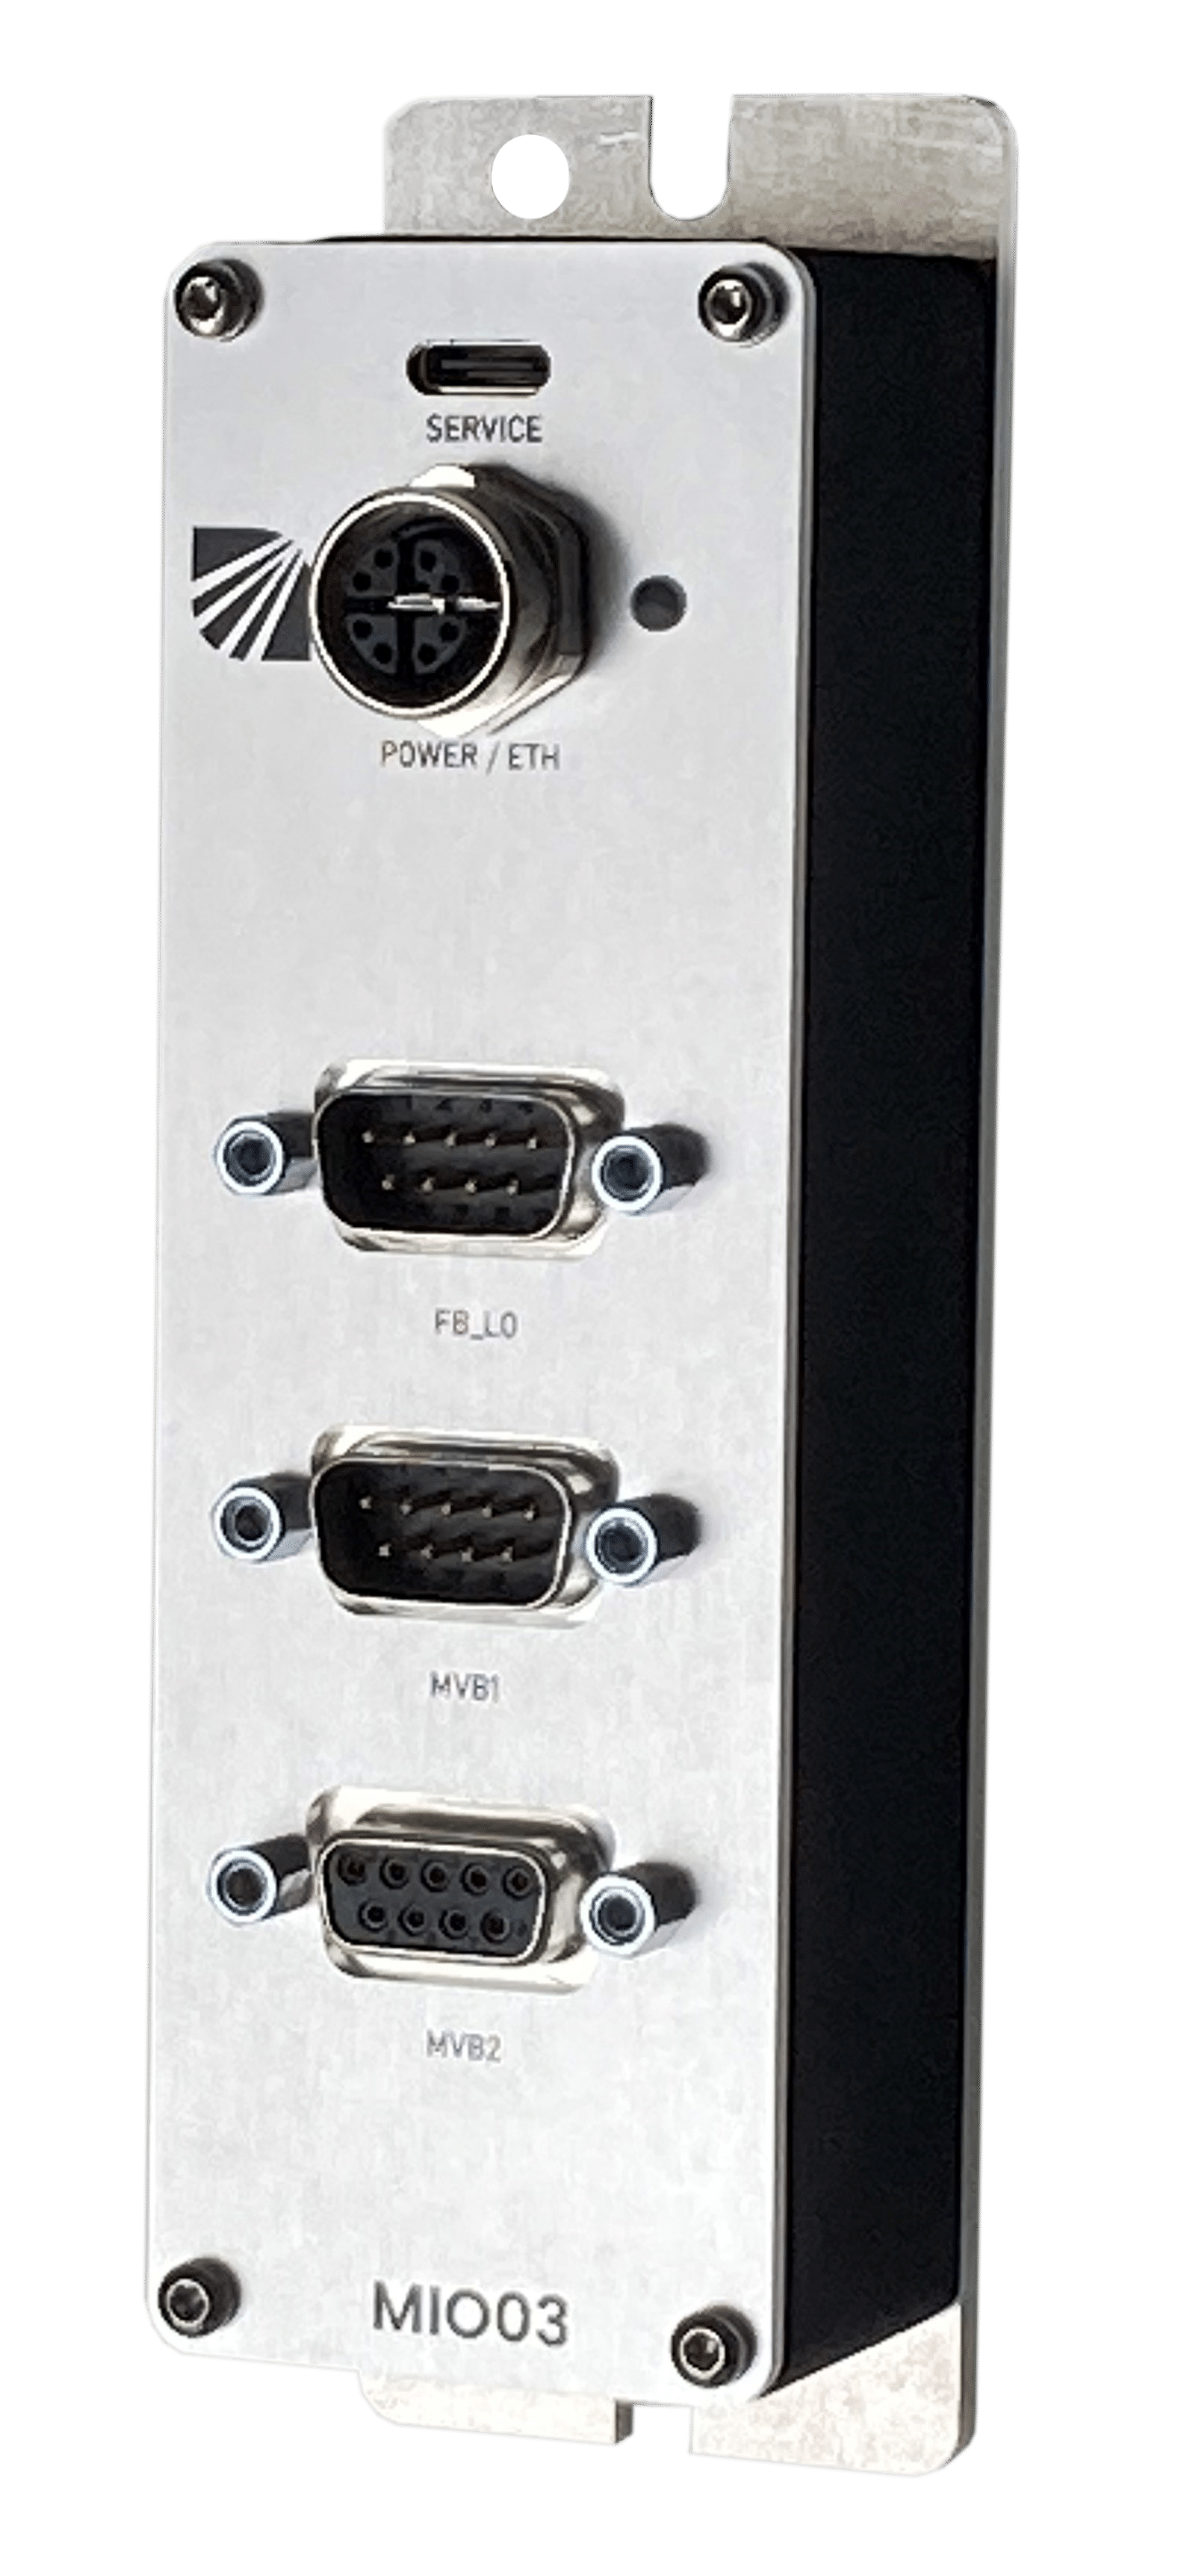
\includegraphics[width=0.2\linewidth]{Figures/Chap3/Konkurenz/CI4Rail.png}
    \caption{Bild von Herstellerseite}
    \label{fig:Ci4RailSniffer}
\end{figure}


%-----------------------------------
% SUBSECTION "Yacer"
%-----------------------------------

\subsection{Konkurenz 3 (Yacer MVB-Analyzer Protocol Analyzer)}
\textcolor{red}{Ebenfalls IP Based}

\begin{figure}[H]
    \centering
    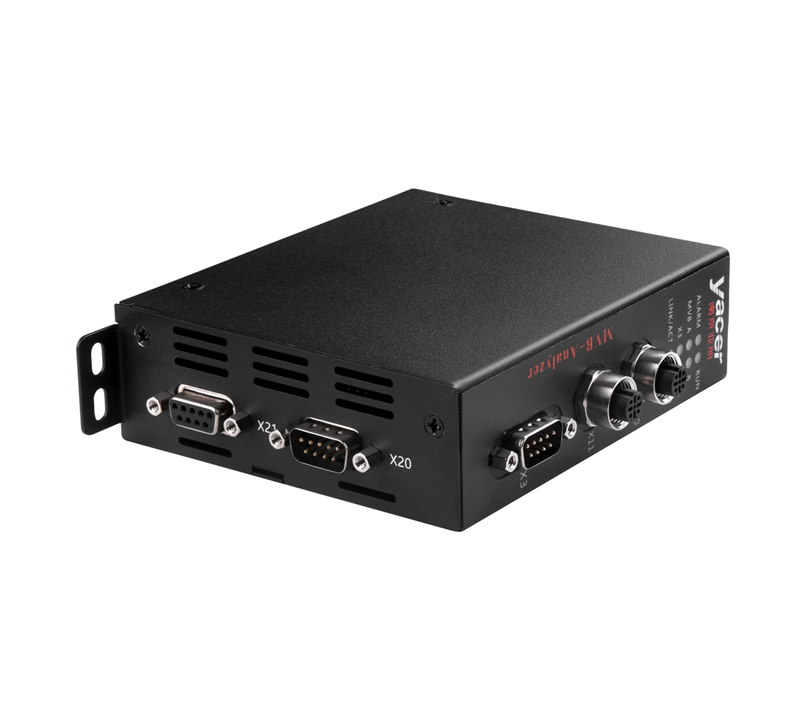
\includegraphics[width=0.5\linewidth]{Figures/Chap3/Konkurenz/Yacer.jpg}
    \caption{Bild von Herstellerseite}
    \label{fig:YacerAnalyzer}
\end{figure}


%-----------------------------------
% SUBSECTION "Abgrenzung"
%-----------------------------------

\subsection{Angrenzung zu den bestehenden Produkten}
\textcolor{red}{Was macht unser Sniffer anders/ besser}

